\documentclass{apuntes}

\title{Teoria de la integral y la medida}
\author{Pedro Valero y Jorge Martín}
\date{14/15 C1}

% Paquetes adicionales
\usepackage{tikztools}
\usepackage{fastbuild}
% --------------------

\begin{document}
\pagestyle{plain}
\maketitle

\tableofcontents
\newpage

\chapter{Sobre la asignatura}
\section{Evaluación}
Hay tres posibles itinerarios de evaluación:
\begin{itemize}
\item \textbf{A}: $\frac{1}{3}T_1+\frac{1}{3}EP+\frac{1}{3}T_2$
\item \textbf{B}: $\frac{2}{5}EP+ \frac{3}{5}EF$
\item \textbf{C}:$EF$
\end{itemize}
Donde $T_1$  y $T_2$ son ``trabajos" que habrá que entregar y se realizará un examen en las fechas indicadas. El ``trabajo" consistirá en la resolución y entrega individual de ciertos ejercicios y el examen se basará en esos ejercicios con algunas variaciones.

\section{Fechas de exámenes}
Las fechas de los exámenes/trabajos serán:
\begin{itemize}
\item $T_1$: 7-Oct
\item $T_2$: 17-Dic
\item $EP$: 10:14-Nov
\item $EF$: 12-Ene
\end{itemize}

\section{Bibliografía}
Durante el curso se seguirán dos libros fundamentalmente:
\begin{enumerate}
\item El libro de Folland: \textit{Real Analysis}
\item El libro de Taylor: \textit{Measure theory and integration} (Serivirá en algunos temas en concreto)
\end{enumerate}

\chapter{Repaso}
\begin{theorem}[Teorema fundamental del Cálculo]
Rellenar. Esto lo completo yo
\end{theorem}

\section{Integral de Riemann}
La construcción de esta integral se realiza sobre un intervalo $[a,b]$, en $\mathbb{R}^2$ y basándonos en una función continua $y=f(x)$.
\begin{defn}[Partición]
Una partición P de $[a,b]$ es una colección finita de subintervalos cerrados $I=i$=$[x_{i-1}, x_i]$ con i=1,2,...,N tal que $a=x_0<x_1<\cdots < x_N=b$.

$\abs{I_i}$ = $x_i-x_{i-1}$
$\abs{P}$=max$\lbrace \abs{I_i} \rbrace$
\end{defn}

Sea $f:[ a,b ] \rightarrow \mathbb{R}$ acotada definimos:
\begin{itemize}
\item \begin{defn}[Suma superior]
$\overline{J}_p(f)=\sum_{i=1}^{N}sup(f(x))|I_i|$
\end{defn}

\item \begin{defn}[Suma inferior]
$\underline{J}_p(f)=\sum_{i=1}^{N}inf(f(x))|I_i|$
\end{defn}
\end{itemize}

La suma inferior de Riemman será la correspondiente a tomar para cada intervalo $[x_{i-1}, x_i]$ la altura mínima de f(x) y construir un rectángulo de dicha altura para posteriormente sumar las áreas de esos rectángulos

La suma superior de Riemann es equivalente a la inferior salvo que en cada intervalo $[x_{i-1}, x_i]$ tomamos la altura máxima de f(x).

La suma superior nos dará un área mayor que el área real encerrada por la curva mientras que la suma inferior nos dará un área menor que la real.

\newpage
\begin{defn}[Finura]
Dadas dos particiones P,Q de [a,b] P es más fina que Q (P$\prec$~Q) si el conjunto de extremos de subintervalos de Q está contenido en el conjunto de extremos de subintervalos de P.

Es decir, P tiene más subintervalos que Q
\end{defn}

Si P$\prec$Q entonces $\overline{J}_P(f) < \overline{J}_Q(f)$  y $\underline{J}_Q(f) < \underline{J}_P(f)$.

Dadas dos particiones $P_1,P_2$ siempre es posible obtener una partición $P$ que refina a ambas. Esta partición será aquella que una todos los extremos de subintervalos de las dos particiones dadas.

Entonces $\underline{J}_{P_1(f)} \leq \underline{J}_P(f) \leq \overline{J}_P(f) \leq \overline{J}_{P_2}$. Es decir, cualquier suma inferior de la función f es menor o igual que cualquier suma superior de dicha función

Por tanto podemos garantizar la existencia de un supremo de las sumas inferiores y un ínfimo de las sumas superiores que serán finitos. Obviamente este ínfimo será mayor que el máximo.

\begin{defn}[Función Integrable\IS Riemann]
una función f:$[ a,b] \rightarrow \mathbb{R}$ acotada es integrable Riemann ($f \in R([a,b])$) si el supremo y el ínfimo anteriores coinciden, en cuyo caso se escribe:
$J(f) = \int_a^b f = \underline{J}(f) = \overline{J}(f) = \int_a^b f(x) dx$
\end{defn}

\subsection{Propiedades}
$f,g \in R([a,b]), \alpha \in \mathbb{R}$
\begin{enumerate}
\item La suma es integrable Riemann
\[f + g \in R([a,b])\]\[ J(f+g) = J(f) + J(g)\]
\item El producto por alfa es integrable Riemann
\[\alpha f \in R([a,b])\] \[ J(\alpha f) = \alpha J(g)\]
\item Si además $f\geq 0$ entonces $J(f)\geq 0$
\item $\forall c \in (a,b)$ $f\in R([a,c])$  y $f\in R([c,b])$ se cumple
$\int_a^b f = \int_a^c f + \int_c^b f$
\end{enumerate}

\begin{example}
Veamos un ejemplo de función acotada en $[ 0,1]$ que NO ES integrable Riemann.
%No se cómo poner el 1 caligráfico
\[
 \ind_{\mathbb{Q}  \cap  [0,1]} (x) =
  \begin{cases}
   1 &  x \in \mathbb{Q} \cap [0,1] \\
   0       &  x \in [0,1] \backslash \mathbb{Q}
  \end{cases}
\]

Para comprobar que esta función no es integrable Riemann tenemos que ver que las sumas inferiores no coinciden con las superiores.
\[\forall P, \overline{J_P}(\ind_{\mathbb{Q} \cap [0,1]}) = 1\]
\[\forall P, \underline{J_P}(	\ind_{\mathbb{Q} \cap [0,1]}) = 0\]


\begin{proof}
La suma inferior da siempre 0 en este caso ya que en cualquier intervalo de la partición hay números irracionales. Por otro lado la suma superior da 1 ya que en todo intervalo hay racionales. Así el ínfimo de las sumas superiores es 1 mientras que el supremo de las sumas inferiores es 0.
\end{proof}
\end{example}

\subsection{Problema de la Integral de Riemann}
Existe una sucesión de funciones $f_n$, tales que $f_n\in R([ 0, 1 ])$, creciente y uniformemente acotada que converge a $f(x)$ tal que:
\[lim \int_0^1 f_n(x) dx \neq \int_0^1 f\]

\begin{example}
%TODO completar esto en condiciones por que da pena.
Sea $\lbrace q_1, q_2, q_3 \cdots \rbrace$ una enumeración los racionales comprendidos entre 0 y 1.

Definimos $f_n(x)=\begin{cases}
   1 &  x \in \lbrace q_1, q_2, q_3 \cdots \rbrace \\
   0       &  x \in [0,1] \backslash \lbrace q_1, q_2, q_3 \cdots \rbrace
  \end{cases}$.
  
El límite de estas funciones sería $f(x)=\begin{cases}
   1 &  x \in \mathbb{Q} \cap [0,1] \\
   0       &  x \in [0,1] \backslash \mathbb{Q}
  \end{cases}$.

Si calculamos las integrales de Riemann superior e inferior vemos que todas las funciones $f_n(x)$ son integrables Riemann pero no lo es $f(x)$, como ya vimos en el ejemplo anterior. Veamos como cada $f_n$ es integrable Riemann:%TODO Añadir etiqueta


Definimos $f_{q_n}(x) =\begin{cases}
	1 & x = q_n\\
	0 & x \in [0,1] \backslash \{q_n\}
	\end{cases}
$

Tomando la partición
$P = \{ [0, q_n - \frac{\varepsilon}{2}], [q_n - \frac{\varepsilon}{2}, q_n + \frac{\varepsilon}{2}], [q_n + \frac{\varepsilon}{2}, 1] \}$

% Dibujo de la recta asociada a la partición
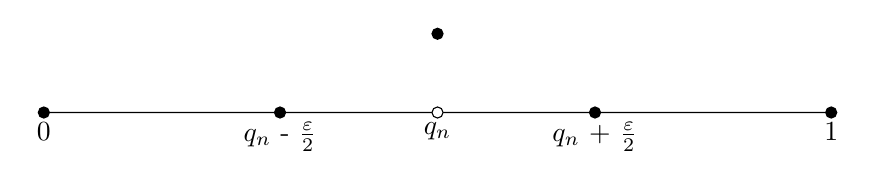
\begin{tikzpicture}
	% Punto (q,1)
	\filldraw (5,1) circle (2pt);	

	% Recta  y puntos
	\filldraw
	(0,0) circle (2pt) node[below]{0} --
	(3,0) circle (2pt) node[below]{$q_n$ - $\frac{\varepsilon}{2}$} --
	(7,0) circle (2pt) node[below]{$q_n$ + $\frac{\varepsilon}{2}$} --
	(10,0) circle (2pt) node[below]{1};
	
	% Recta de ceros
	\draw (0,0) -- (10,0);
	
	% Punto (q,0)
	\filldraw[color=white, draw=black] (5,0) circle (2pt) node[below, text=black]{$q_n$};	
\end{tikzpicture}

Podemos ver que $f_{q_n}$ es integrable Riemman, ya que:
\[\overline{J}_P (f_{q_n}) = \varepsilon \Rightarrow \overline{J} (f_{q_n}) = 0 = \underline{J} (f_{q_n})\]

Como $f_n = f_{q_1} + \ldots + f_{q_n}$, y toda $ f_{q_i}$ es integrable Riemann, por la propiedad 1 sabemos que $f_n$ será integrable Riemann.
\end{example}

\begin{defn}[Contenido]
A toda integral sobre un intervalo se puede asociar una forma de medir subconjuntos del intervalo.

En el caso de la integral de Riemann esa ``medida" suele llamarse contenido de Jordan.

Sea C$\subset$[a,b] se define:
\[cont(C) = \int_a^b \ind_{C}(x) dx\]
siempre que $\ind_C \in R([a,b])$

En general, aunque $\ind_C \notin R([a,b])$ se puede hablar de contenido exterior y de contenido interior:
\[cont^+(C)=\overline{J(\ind_C)}\]
\[cont^-(C)=\underline{J(\ind_C)}\]

Suele decirse que un conjunto ``tiene contenido" $cont^+(C)=cont^-(C)$
\end{defn}

El problema que abordaremos próximamente es que la unión numerable de conjuntos con contenido no siempre tiene contenido.

\obs $f\in R([a,b]) \Leftrightarrow \forall \epsilon \exists P \tq \overline{J_P(f)}-\underline{J_P(f)} < \epsilon$


\textbf{En moodle hay un resumen de este tema}

\begin{example}
\textbf{Ejercicio 1 de la hoja 1}

El objetivo del ejericio es demostrar que $f\in R([a,b]) \Rightarrow \abs{f}\in R([a,b])$

Para ellos definimos: 
$f^+(x) = max\lbrace f(x), 0 \rbrace$

$f(x) = f^+(x) - f^-(x)$

De donde podemos deducir:

$f^-(x) = f^+(x)-f(x)=max \lbrace -f(x), 0 \rbrace$

Y las funciones tienen el siguiente aspecto:

\begin{center}
% Funcion f
\begin{tikzpicture}
	% Ejes
	\draw (0,3) -- (0,-2);
	\draw (-1,0) -- (4,0);
	\draw (0.5,0) -- (0.5,-0.1) node[below] {a};
	\draw (3,0) -- (3,-0.1) node[below] {b};

	\draw [domain=0.5:3, samples=50, very thick] plot (\x, {2 * cos(\x r)});
	\draw (0.5 * pi, 1) node{f};
	\coordinate (a) at (0.5,0);
	\coordinate (b) at (0.3,0);
\end{tikzpicture}

% Funcion f+
\begin{tikzpicture}
	% Ejes
	\draw (0,3) -- (0,-2);
	\draw (-1,0) -- (4,0);
	\draw (0.5,0) -- (0.5,-0.1) node[below] {a};
	\draw (3,0) -- (3,-0.1) node[below] {b};
	
	\draw[domain=0.5:0.5 * pi, samples=50, very thick] plot (\x, {2 * cos(\x r)});
	\draw[very thick] (0.5 * pi, 0.03) -- (3,0.03);
	\draw (0.5 * pi, 1) node{$f^+$};
	\coordinate (a) at (0.5,0);
	\coordinate (b) at (0.3,0);
\end{tikzpicture}

% Funcion f-
\begin{tikzpicture}
	% Ejes
	\draw (0,3) -- (0,-2);
	\draw (-1,0) -- (4,0);
	\draw (0.5,0) -- (0.5,-0.1) node[below] {a};
	\draw (3,0) -- (3,-0.1) node[below] {b};
	
	\draw[domain=0.5 * pi:3, samples=50, very thick] plot (\x, {2 * cos(\x r)});
	\draw[very thick] (0.5,0.03) -- (0.5 * pi, 0.03);
	\draw (0.5 * pi, 1) node{$f^-$};
	\coordinate (a) at (0.5,0);
	\coordinate (b) at (0.3,0);
\end{tikzpicture}
\end{center}


%\caption{La bola verde ($\bola(y, r-\dst(x,y)$) contenida dentro de $\bola(x, r)$.}
%\label{figBolaContenida}


Así podemos escribir 
$\abs{f(x)} = f^+(x)+f^-(x)$.

Gracias a esta afirmación el problema se reduce a demostrar que la parte positiva ($f^+$ ) es integrable Riemann, ya que entonces lo serán  y $f^-$  y $\abs{f(x)}$  por ser la suma/resta de dos funciones integrables Riemann.


Vamos a calcular $f^+(x)$:
\[\overline{J_P(f^+)}-\underline{J_P(f^+)} = \sum_{k=1}^n\left(\sup_{x\in I_k}(f^+(x))\right)\abs{I_k} - \sum_{k=1}^n\left(\underset{x\in I_k}{inf}(f^+(x))\right)\abs{I_k}=\]
\[= \sum_{k=1}^n\left(\sup_{x\in I_k}(f^+(x))-\underset{x\in I_k}{inf}(f^+(x))\right)\abs{I_k} \leq
\sum_{k=1}^n\left(\sup_{x\in I_k}(f(x))-\underset{x\in I_k}{inf}(f(x))\right)\abs{I_k} =\] \[=\overline{J_P(f)}-\underline{J_P(f)} = 0\]

Y sabemos que f es integrable
\end{example}

\begin{example}
\textbf{Ejercicio 2 hoja 1}

El ejercicio nos pide demostrar: $f,g \in R([a,b]), h(x) = max\lbrace f(x), g(x) \rbrace \Rightarrow h \in R([a,b])$

Vamos a comprobar que la diferencia entre las integrales Riemann superior e inferior es 0.
Pero antes fijémonos en la \underline{indicación}:

\[\sup\big\{ \max\{f(x), g(x)\}\big\} - inf\big\{ \max\{f(x), g(x)\} \big\} \leq \]

\[ \leq \max\big\{ \sup_{x \in I_k} (f(x)) - \underset{x \in I_k}{inf} (f(x)), \sup_{x \in I_k} (g(x)) - \underset{x \in I_k}{inf} (g(x)) \big\} \leq \]

\[ \leq \left(\sup_{x \in I_k} (f(x)) - \underset{x \in I_k}{inf} (f(x))\right) + \left(\sup_{x \in I_k} (g(x)) - \underset{x \in I_k}{inf} (g(x))\right) \]


Ahora podemos probar que:
\[\overline{J_P(h)}-\underline{J_P(h)}
= \sum\left(\sup_{x\in I_k}(h(x))-\underset{x\in I_k}{inf}(h(x))\right)\abs{I_k} \leq\]

\[\leq \sum\left( \sup_{x \in I_k} (f(x)) - \underset{x \in I_k}{inf} (f(x)) \right) \abs{I_k} + 
 \sum\left( \sup_{x \in I_k} (g(x)) - \underset{x \in I_k}{inf} (g(x)) \right) \abs{I_k} \]
\end{example}
\end{document}



